% =====================================================================
%  Seance 2 -- A. garde, plan, ou vivent les donnees (frames 1--9)
% =====================================================================
\section{Séance 2 --- Données d'infrastructures et préparation}
\chapterslide{Séance 2}{Données d'infrastructures et préparation des données}
{4 h --- 2 h cours / 2 h TP --- Partie 2 du syllabus EPD-GIT-5534}
{\textbf{Objectifs :} connaître les sources de données d'une infrastructure et
leurs pièges (granularité, horloges) $\bullet$ maîtriser le nettoyage :
doublons, valeurs manquantes, valeurs aberrantes $\bullet$ construire des
\textbf{signaux} (fenêtres, p99, encodage cyclique) $\bullet$ produire le
\textbf{jeu de données supervisé} du dossier (étiquette « incident $\le$ 30 min »).}

\begin{frame}{Plan de la séance (4 h)}
\begin{columns}[t]
\begin{column}{0.48\textwidth}
\begin{kbox}[Cours magistral --- 2 h]
\begin{enumerate}
\item \textbf{Où vivent les données} (40 min) : métriques, journaux, événements,
traces --- granularités et horloges.
\item \textbf{Préparer les données} (60 min) : doublons, manquants, aberrants,
rééchantillonnage.
\item \textbf{Ingénierie de signaux} (20 min) : fenêtres, p99, encodage cyclique,
dérive de capteur.
\end{enumerate}
\end{kbox}
\end{column}
\begin{column}{0.48\textwidth}
\begin{ebox}[Travaux pratiques --- 2 h]
\textbf{« Du brut au dataset supervisé »} sur \file{nosys\_metriques\_brutes.csv} :
\begin{enumerate}
\item B1 --- audit des défauts (30 min)
\item B2 --- nettoyage : doublons, NaN, aberrants (35 min)
\item B3 --- signaux : fenêtres, p99, encodage cyclique (30 min)
\item B4 --- étiquette « incident $\le$ 30 min » (35 min)
\item B5 --- livrable : \file{nosys\_features.csv} + dictionnaire (10 min)
\end{enumerate}
\end{ebox}
\end{column}
\end{columns}
\vspace{1mm}
\begin{center}\small
Nouveau fichier du dossier : la \textbf{collecte brute} avec ses défauts réels ---
le TP part du brut, pas du propre.
\end{center}
\end{frame}

\begin{frame}{Où vivent les données d'une infrastructure ?}
\begin{center}
\small
\begin{tabular}{@{}p{2.3cm}p{4.6cm}p{2.6cm}p{3.6cm}@{}}
\toprule
\textbf{Source} & \textbf{Contenu} & \textbf{Granularité} & \textbf{Exemple}\\
\midrule
\textbf{Métriques} & séries temporelles numériques & 10 s -- 5 min &
Prometheus, SNMP, agents (notre \py{cpu\_pct})\\
\addlinespace[1pt]
\textbf{Journaux} & événements textuels datés & à l'événement &
syslog, ELK (\file{nosys\_logs.csv})\\
\addlinespace[1pt]
\textbf{Événements} & alertes, déploiements, incidents & ponctuel &
PagerDuty, webhooks (\py{alarme})\\
\addlinespace[1pt]
\textbf{Traces} & parcours d'une requête entre services & par requête &
OpenTelemetry, Jaeger\\
\addlinespace[1pt]
\textbf{Tickets} & interventions humaines, causes & ponctuel &
ServiceNow, Jira --- la « vérité terrain »\\
\bottomrule
\end{tabular}
\end{center}
\vspace{1mm}
\begin{kbox}[La règle d'or du ML applicatif]
Un bon modèle d'infrastructure \textbf{joint} plusieurs sources :
métriques (le symptôme) + événements (le contexte) + tickets (la cause).
La séance 2 construit cette jointure.
\end{kbox}
\end{frame}

\begin{frame}{Granularité et horloges : les pièges silencieux}
\begin{columns}[t]
\begin{column}{0.5\textwidth}
\begin{block}{Granularité hétérogène}
Dans notre collecte brute, \textbf{srv-07 relève toutes les 15 min} alors
que les 7 autres relèvent toutes les 5 min (config d'agent différente).
\begin{itemize}
\item Une jointure naïve sur l'horodatage \textbf{perd} les données srv-07.
\item Il faut \textbf{rééchantillonner} vers une grille commune (séance : f09).
\end{itemize}
\end{block}
\begin{block}{Horloges}
\begin{itemize}
\item Tout serveur n'a pas la même heure (dérive NTP, fuseaux).
\item Règle : collecter en \textbf{UTC}, convertir à l'affichage.
\item Un décalage de 2 min entre deux sources détruit une jointure à la minute.
\end{itemize}
\end{block}
\end{column}
\begin{column}{0.46\textwidth}
\begin{wbox}[Le défaut que personne ne voit]
Pas de valeur manquante affichée, pas d'erreur : \textbf{juste moins de
points}. Un compte de lignes par serveur révèle la granularité :
srv-07 a 2\,880 points au lieu de 8\,640.
\end{wbox}
\begin{qbox}[Question]
Vous jointez métriques (5 min) et logs (à l'événement). Pourquoi une
jointure \py{merge} exacte échoue presque toujours ?\\
(a) les logs sont trop nombreux \quad (b) les horodatages ne coïncident
jamais exactement --- il faut \textbf{as-of join} / fenêtres \quad
(c) il faut du SQL
\end{qbox}
\end{column}
\end{columns}
\end{frame}

\begin{frame}{Le fichier du TP : une collecte « comme en production »}
\footnotesize%
\begin{columns}[t]
\begin{column}{0.52\textwidth}
\begin{ebox}[\file{nosys\_metriques\_brutes.csv} --- 63 521 lignes]
Les défauts semés (graine 5534, script \file{make\_nosys\_s2.py}) :
\begin{itemize}
\item \textbf{200 lignes dupliquées} (ré-tentative réseau).
\item \textbf{5 508 valeurs manquantes} (1,73 \% des cellules numériques) ---
capteur flottant.
\item \textbf{12 valeurs aberrantes} : température à \textbf{1 575 °C},
CPU à \textbf{350 \%} --- pic de capteur, pas d'incident.
\item \textbf{6 trous} de 15 à 40 min (agent redémarré).
\item \textbf{srv-07 en granularité 15 min}.
\item \textbf{srv-06 : capteur de température qui dérive}.
\end{itemize}
\end{ebox}
\end{column}
\begin{column}{0.44\textwidth}
\begin{center}
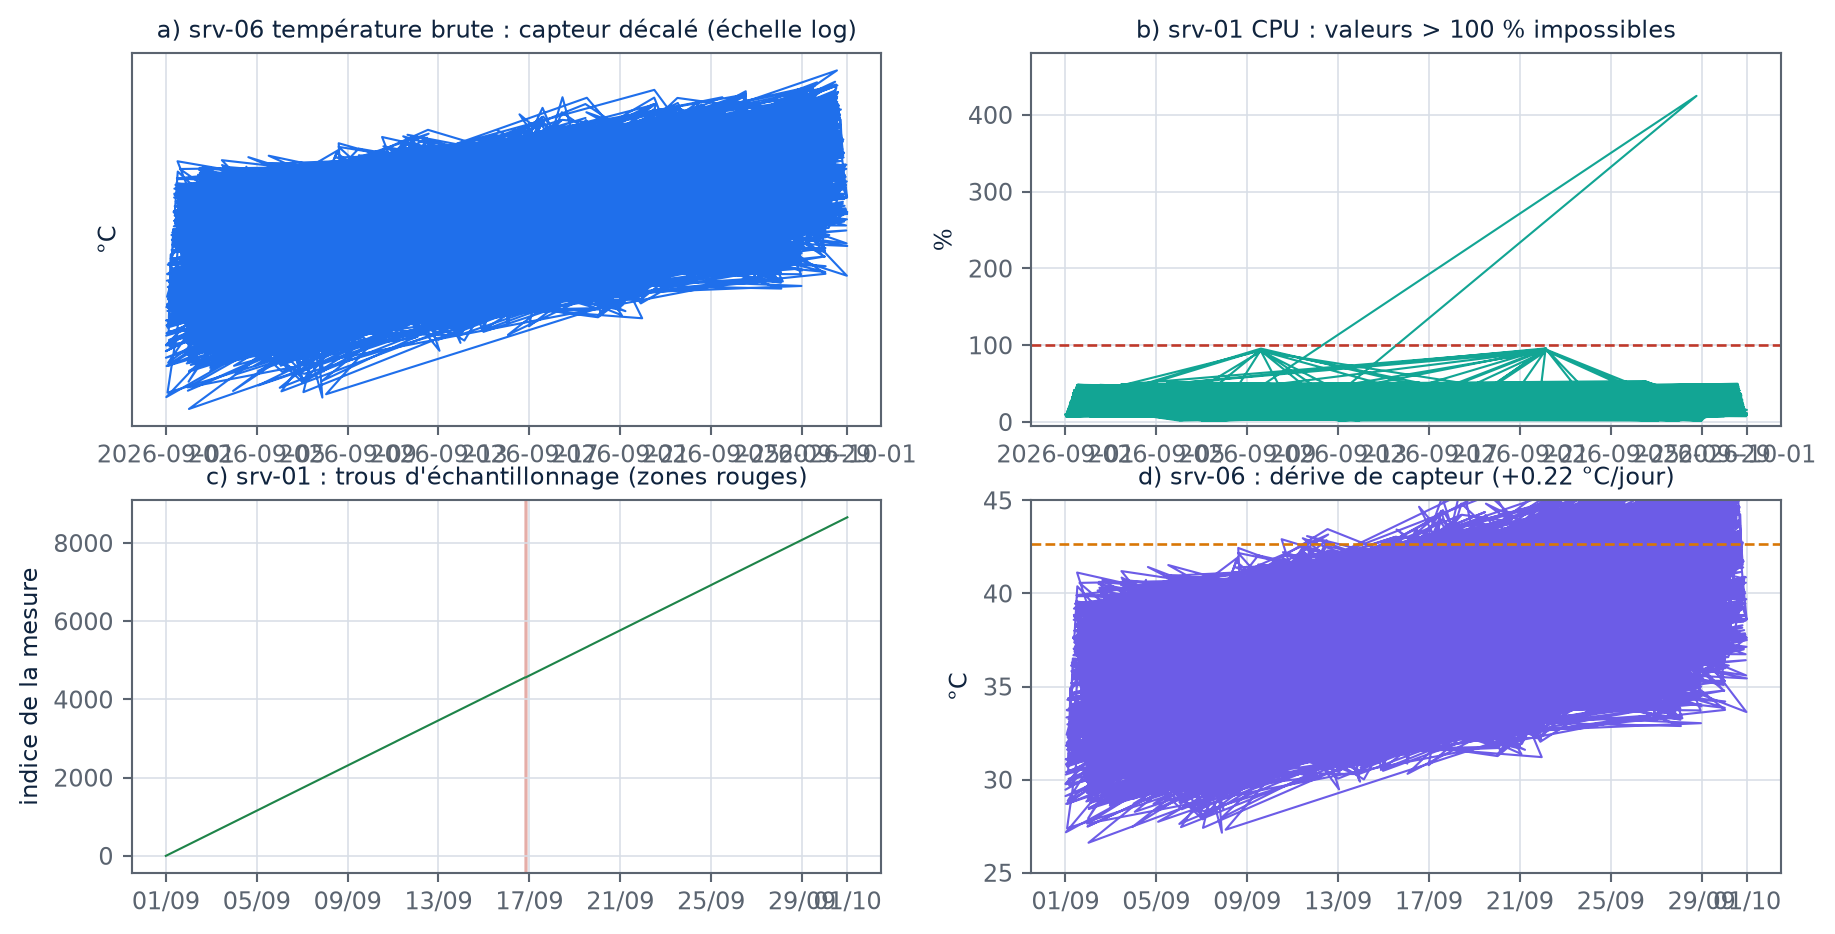
\includegraphics[width=\textwidth]{f08_defauts.png}
\end{center}
\end{column}
\end{columns}
\end{frame}

\begin{frame}{Quiz 1 --- les sources (5 min)}
\begin{qbox}[3 questions]
\begin{enumerate}
\item Quelle source donne la \textbf{cause} d'un incident (et pas seulement le symptôme) ?\\
(a) les métriques \quad (b) les tickets et journaux d'intervention \quad
(c) les traces
\item srv-07 relève toutes les 15 min. Sur un mois, il produit :\\
(a) 8 640 points \quad (b) 2 880 points \quad (c) 28 800 points
\item Le pire défaut d'une jointure métriques/logs naïve est :\\
(a) elle est lente \quad (b) les horodatages ne coïncident jamais exactement
$\Rightarrow$ presque tout est perdu \quad (c) elle crée des doublons
\end{enumerate}
\end{qbox}
\vspace{1mm}
\begin{solbox}[Réponses]
\textbf{1 : b} \quad \textbf{2 : b} (288/jour $\times$ 30) \quad \textbf{3 : b} ---
d'où les jointures par \textbf{fenêtre} (as-of / \py{merge\_asof}).
\end{solbox}
\end{frame}
